 \section{Manifestaciones seguras}

En una decisión temeraria una ciudad decidió autorizar un conjunto de n manifestaciones el mismo día y horas. Cada manifestación comienza en un punto de reunión y tiene un destino final. Para evitar enfrentamientos y confusiones desean que cada ruta sea aislada de las otras. Contamos con el mapa de la ciudad que incluye todos los caminos e intersecciones por lo que pueden ir las marchas. Nos piden que elaboremos un algoritmo que retorne los caminos a seguir para cada manifestación de modo que no haya riesgo de un cruce (si es posible).\newline
Debemos demostrar que es un problema NP-Completo.
%=============================================

\subsection{Solución}
El problema que precede se puede modelar con un grafo en donde los nodos son las intersecciones de las calles y las aristas son las calles de la ciudad. En un principio todas las calles están disponibles para efectuar las manifestaciones siempre y cuando no se superpongan las manifestaciones.
%=============================================

\subsection{Demostración NP-Completo}
Para demostrar que es $\mathsf{NP-Completo}$ debemos demostrar que nuestro problema pertenece a $\mathsf{NP}$ y a $\mathsf{NP-Hard}$ simultáneamente.

\subsubsection{Demostración NP}
Para demostrar que el problema es $\mathsf{NP}$ debemos poder corroborar la solución propuesta en tiempo polinomial. Usando la analogía de la cerradura y la llave, esto sería equivalente a dada la llave probar que esta abre la cerradura en "tiempo polinomial". \newline

A continuación se propone un algoritmo que verifica la solución propuesta en tiempo polinomial:

\begin{verbatim}
Llamar L a la lista de manifestaciones(representadas por tuplas de nodos)

Funcion esManifestacionValida(L):
    Llamar visitados a la lista que contendrá a los nodos visitados
    
    visitados es lista vacia
    Para cada manifestacion en manifestaciones:
        Para cada esquina en manifestacion:
            Si esquina en visitados:
                Devolver falso
            Sino:
                visitados agregar esquina
    Devolver verdadero
\end{verbatim}

Se puede apreciar que la complejidad es de $\mathcal{O}(km)$ siendo $k$ la cantidad de manifestaciones y $m$ la cantidad máxima de esquinas atravesadas por una manifestación.

\subsubsection{Demostración NP-Hard}
Para demostrar que el problema es $\mathsf{NP-Hard}$, consideremos una instancia del problema conocido como conjunto independiente que consiste en un grafo $G=(V, E)$ con $|V|=n$ y un valor entero $k$.

\begin{figure}[H]
\centering
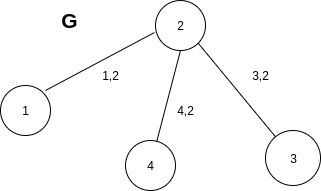
\includegraphics[width=0.9\textwidth]{Informe/Imagenes/Parte1/grafico 1.png}
\caption{\label{fig:class01}Instancia conjunto independiente}
\end{figure}

Sea el grafo $M = (V', E')$ donde $V' = V \cup \{ x_{u,v} \, : \, (u,v) \in E \}$ y $E' = V' \times (V'-1)$.

\begin{figure}[H]
\centering
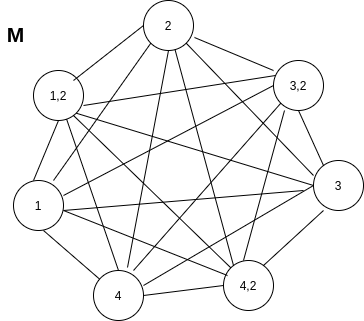
\includegraphics[width=0.9\textwidth]{Informe/Imagenes/Parte1/grafico 2.png}
\caption{\label{fig:class01}Grafo manifestaciones}
\end{figure}

Para cada $u \in V$ siendo $v_1, v_2, \dots, v_m$ los vecinos de $u$ en $G$ y definamos la ruta $P_u = \langle u, x_{u,v_1}, x_{u,v_2}, \dots, x_{u,v_m} \rangle⟩$ en $M$. Siendo $\mathcal{P} = \{P_u \, : \, u \in V\}$.\newline

Hay un conjunto independiente de tamaño como máximo $k$ en $G$, si y solo si hay un subconjunto $\mathcal{P}'$ con $|\mathcal{P}'| \le k$ tal que los caminos en $\mathcal{P}'$ son vértices disjuntos de a pares.

\begin{figure}[H]
\centering
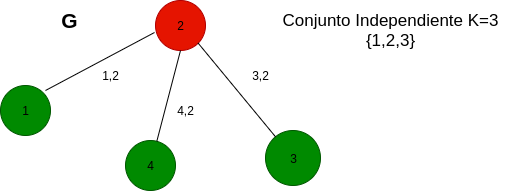
\includegraphics[width=0.9\textwidth]{Informe/Imagenes/Parte1/grafico 4.png}
\caption{\label{fig:class01}Nodos independientes}
\end{figure}

Más precisamente, si $S$ es un conjunto independiente de $G$, entonces $\{ P_u \, : \, u \in S \}$ es una colección de caminos separados de vértices por pares en $M$ y, si $\mathcal{P}'$ es una colección de caminos separados de vértices por pares en $M$, entonces $\{u \, : \, P_u \in \mathcal{P}' \}$ es un conjunto independiente de $G$.

\begin{figure}[H]
\centering
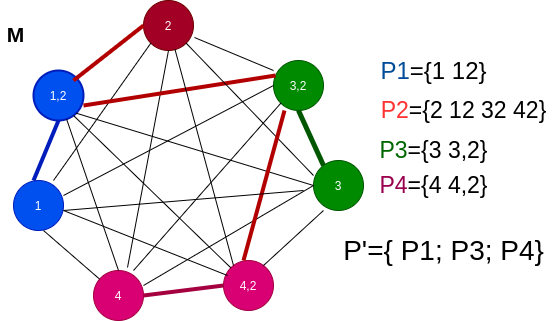
\includegraphics[width=0.9\textwidth]{Informe/Imagenes/Parte1/grafico 3.png}
\caption{\label{fig:class01}Rutas}
\end{figure}

\begin{figure}[H]
\centering
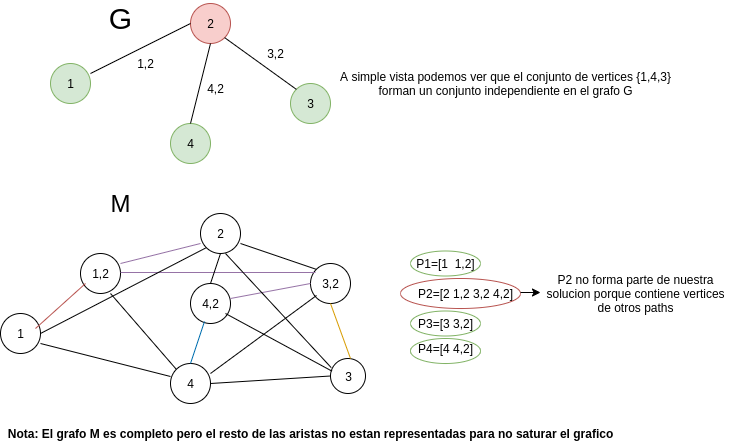
\includegraphics[width=0.9\textwidth]{Informe/Imagenes/Parte1/grafico 5.png}
\caption{\label{fig:class01}Demostración NP-Completo}
\end{figure}
%=============================================


